\begin{figure}
	\centering
	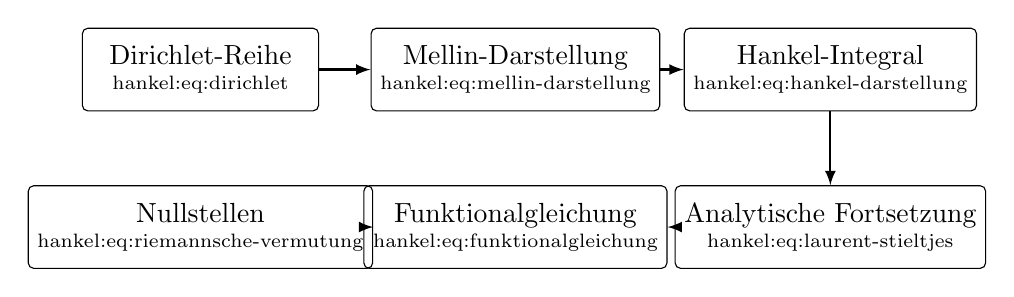
\begin{tikzpicture}[
		block/.style={
			draw,
			rounded corners=2pt,
			minimum width=3.0cm,
			minimum height=1.05cm,
			align=center
		},
		arrow/.style={->,thick,>=latex}
		]
		\node[block] (d) at (0,0)
		{Dirichlet-Reihe\\[-1mm]
			{\scriptsize\eqref{hankel:eq:dirichlet}}};
		
		\node[block] (m) at (4,0)
		{Mellin-Darstellung\\[-1mm]
			{\scriptsize\eqref{hankel:eq:mellin-darstellung}}};
		
		\node[block] (h) at (8,0)
		{Hankel-Integral\\[-1mm]
			{\scriptsize\eqref{hankel:eq:hankel-darstellung}}};
		
		\node[block] (a) at (8,-2)
		{Analytische Fortsetzung\\[-1mm]
			{\scriptsize\eqref{hankel:eq:laurent-stieltjes}}};
		
		\node[block] (f) at (4,-2)
		{Funktionalgleichung\\[-1mm]
			{\scriptsize\eqref{hankel:eq:funktionalgleichung}}};
		
		\node[block] (n) at (0,-2)
		{Nullstellen\\[-1mm]
			{\scriptsize\eqref{hankel:eq:riemannsche-vermutung}}};
		
		\draw[arrow] (d) -- (m);
		\draw[arrow] (m) -- (h);
		\draw[arrow] (h) -- (a);
		\draw[arrow] (a) -- (f);
		\draw[arrow] (f) -- (n);
	\end{tikzpicture}
	
	\caption{Der rote Faden des Kapitels.}
	\label{hankel:fig:uebersicht}
\end{figure}
